\section*{Introduction} %Improve and rewrite for future developments of the project
\label{sec:introduction}

    Volume discounts on products make it very valuable to find a way to form coalitions. Within buyer coalition formation, there are many different problems and trade-offs for developing a good strategy. One of the main problems is that different participating parties can have different preferences which are usually not known to everyone. How soon should a buyer concede? And can he or she for example base its conceding strategy on his or her buying power? 

    In this assignment, a modular agent was developed that can participate in buyer coalition formation negotiations and the more general MOPaC protocol, the Multiple Offers Protocol for Multilateral Negotiations with Partial Consensus.

    \subsection*{Description of MOPaC}

        The MOPaC protocol allows two or more parties to negotiate on different issues and reach a partial consensus, where not all parties are required to agree. This makes MOPac more flexible than traditional multiparty negotiation protocols such as SAOP.
        A MOPaC negotiation consists of individual rounds with multiple phases; the bidding phase, the voting phase and the opt-in phase. These phases are described in further detail in \autoref{sec:strategies}.

    \subsection*{Description of the buyers coalition formation}

        A group shopping market may offer multiple items to buyers for subsequent buyer coalition formations. In this case, in order to reduce the price of items, buyers tend to form a large group to buy one type of item. As long as the size of the group reaches a specific number, this group can obtain a relatively low price. With a sufficient number of customers, the sellers are willing to provide lower prices which attracts people to form a buyer coalition.

    \subsection*{The reason why MOPaC fits the Buyer coalition formation problem}

        In an e-marketplace, buyers often have the choice between several products. Each buyer represents one agent in the negotiation, and they aim to maximize their benefit. As for the buyer coalition formation part, this formation does not require a full consensus of all the buyers. In this case, the MOPaC protocol perfectly fits the buyer coalition formation problem.

        In the MOPaC negotiation, one of the most important things for a party is its "power". This represents how much influence the party has in the negotiation, which in the case of this buyer coalition formation problem represents the amount of products the party wants to buy. 

        \autoref{fig:galaxy} shows an example for a buyer group using the MOPaC protocol. A circle represents one buyer while size represents its demanded amount of products or power. The buyers in the same formation have the same color. Parties not yet in a coalition might have different preferences, but they can still join into an existing formation or make a new one to persuade other buyers to join it during the negotiation. 

        \begin{figure}[htp]
            \centering
            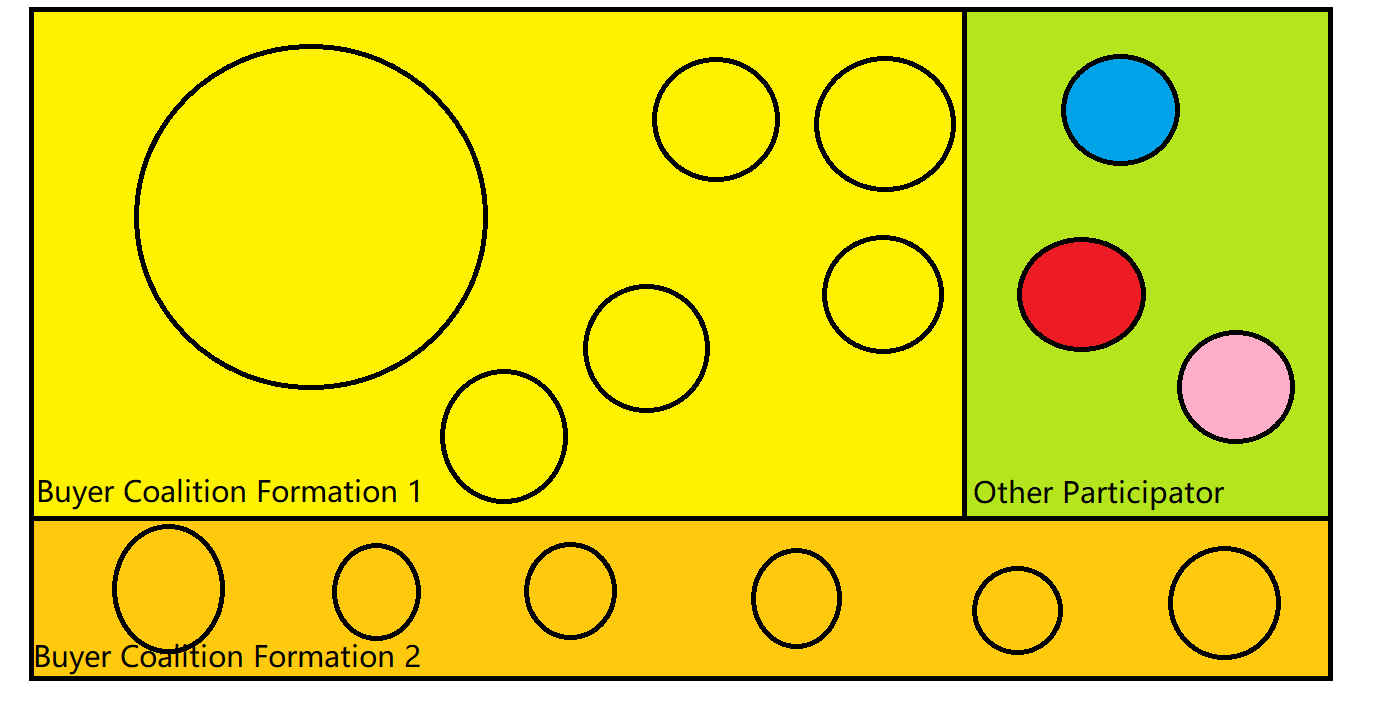
\includegraphics[width=10cm]{figures/Predicted Outcome Example.png}
            \caption{An image of a predicted outcome}
            \label{fig:galaxy}
        \end{figure}

    In \autoref{sec:preferenceprofiles} ,the preference profiles of the different buyers will be discussed. In \autoref{sec:strategies}, the different possible bidding and conceding strategies for the buyers will be discussed, together with possible extensions. 




